% Created 2016-03-23 Wed 11:37
\documentclass[bigger]{beamer}
\usepackage[utf8]{inputenc}
\usepackage[T1]{fontenc}
\usepackage{fixltx2e}
\usepackage{graphicx}
\usepackage{longtable}
\usepackage{float}
\usepackage{wrapfig}
\usepackage{rotating}
\usepackage[normalem]{ulem}
\usepackage{amsmath}
\usepackage{textcomp}
\usepackage{marvosym}
\usepackage{wasysym}
\usepackage{amssymb}
\usepackage{hyperref}
\tolerance=1000
\usetheme{default}
\author{Weston Dransfield}
\date{\today}
\title{Cellular Automata}
\hypersetup{
  pdfkeywords={},
  pdfsubject={},
  pdfcreator={Emacs 24.5.1 (Org mode 8.2.10)}}
\begin{document}

\maketitle
\begin{frame}{Outline}
\tableofcontents
\end{frame}


\begin{frame}[label=sec-1]{The Basics}
\begin{itemize}
\item<1-> Spacial Structure
\item<2-> Local Interactions
\item<3-> Cell State
\item<4-> Cell Transitions
\end{itemize}
\end{frame}

\begin{frame}[label=sec-2]{Spacial Structure}
\begin{itemize}
\item<1-> Grid - Like a city
\item<2-> Agents - Like a home in the city
\end{itemize}
\end{frame}

\begin{frame}[label=sec-3]{Spacial Structure}

\includegraphics[width=7cm]{images/grid.png}
\end{frame}

\begin{frame}[label=sec-4]{Local Interactions}
Agents may only interact with a set number of agents around them. This region is called a neighborhood.
\begin{itemize}
\item<1->Von Neumann neighborhood (most local).
\item<2->Moore neighborhood (less local).
\item<3->\(n*n\) Moore neighborhood for \(n > 3\) (least local).
\end{itemize}
\pause
\pause
\pause
Locality indicates how many agents a single agent interacts with. High locality indicates more interactions (Think of how a rumor spreads).
\end{frame}

\begin{frame}[label=sec-5]{Local Interactions}

\includegraphics[width=7cm]{images/grid.png}
\end{frame}

\begin{frame}[label=sec-6]{Cell State}
Cells have a state
\begin{itemize}
\item<1->Binary
\item<2->Any number of states
\end{itemize}
\end{frame}

\begin{frame}[label=sec-7]{Cell Transitions}
CA have discrete chunks of time called rounds. Each round produces the next "generation" of cells.
\end{frame}

\begin{frame}[label=sec-8]{Cell Transitions}
The next state of a cell is a function of:
\begin{itemize}
\item<1->It's current state
\item<2->The state of cells in its neighborhood
\end{itemize}
\pause
\pause
Think of your opinion on a topic changing by being surrounded by people with a different view.
\end{frame}

\begin{frame}[label=sec-9]{Elementary Cellular Automaton}
What is the simplest...
\begin{itemize}
\item<1->Grid of cells?
\item<2->Useful number of states?
\item<3->Neighborhood?
\end{itemize}
\end{frame}

\begin{frame}[label=sec-10]{Elementary Cellular Automaton}
What is the simplest...
\begin{itemize}
\item<1->Grid of cells - an array
\item<1->Useful number of states - binary
\item<1->Neighborhood - 2 adjacent cells of the agent
\end{itemize}
\end{frame}

\begin{frame}[label=sec-11]{Elementary Cellular Automaton}
How do we describe the state of cell \(c_t\) as a function of the neighbors of \(c_t\) at time \(t-1\)?
\begin{itemize}
\item<1->There are \(2^3 = 8\) neighborhood combinations for any given neighborhood.
\item<2->Simply create an assignment for each combination!
\item<3->This assignment is called a rule set (how many possible rule sets?)
\end{itemize}
\end{frame}

\begin{frame}[label=sec-12]{Example Program}
\url{https://github.com/westonkd/Completeness/tree/CA}
\end{frame}

\begin{frame}[label=sec-13]{2D CA Example - Conway's Game of Life}
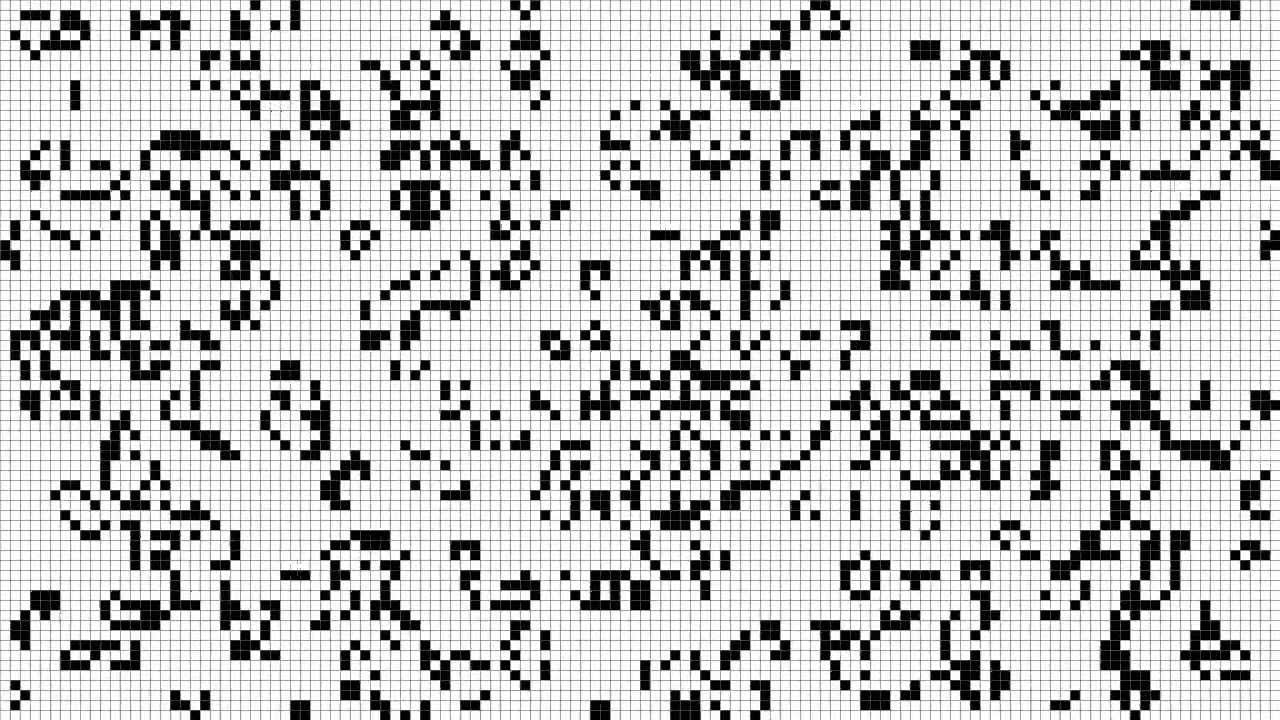
\includegraphics[width=11cm]{images/gol1.jpg}
\end{frame}

\begin{frame}[label=sec-14]{Conway's Game of Life}
\begin{enumerate}
\item<1->Rules
\item<2->Entities
\item<3->Results
\item<4->Computational tidbits
\end{enumerate}
\end{frame}

\begin{frame}[label=sec-15]{Conway's Game of Life Rules}
\begin{itemize}
\item<1->2 states - dead or alive
\item<2->3x3 Moore neighborhood
\end{itemize}

\begin{enumerate}
\item<3->Any live cell with fewer than two live neighbors dies (under population).
\item<4->Any cell with 2 or 3 live neighbors lives on to the next generation.
\item<5->A cell with more than 3 live neighbors dies (over crowding).
\item<6->A dead cell with exactly 3 live neighbors becomes alive (reproduction).
\end{enumerate}
\end{frame}

\begin{frame}[label=sec-16]{Examples}
\end{frame}
\begin{frame}[label=sec-17]{Conway's Game of Life Entities}
\begin{enumerate}
\item<1->Still lives - entity stays the same throught generations
\item<2->Oscillators - entity changes shape and returns to original position (periods)
\item<3->Spaceships - Moving oscillators
\end{enumerate}
\url{https://en.wikipedia.org/wiki/Conway\%27s_Game_of_Life}
\end{frame}
\begin{frame}[label=sec-18]{Conway's Game of Life Results}
\begin{enumerate}
\item<1->Fade away completely
\item<2->Stable configuration
\item<3->Oscillating phase
\end{enumerate}
\end{frame}
\begin{frame}[label=sec-19]{Conway's Game of Life Decidability}
The question - "Given a starting pattern and an ending pattern, will the starting pattern ever reach the ending pattern?"
\begin{itemize}
\item<2->Undecidable - halting problem
\item<3->"Indeed, since the game of life includes a pattern that is equivalent to a UTM (universal Turing machine), this "deciding" algorithm, if existed, could have been used to solve the halting problem, by taking the initial pattern as the one corresponding to a UTM+input and the later pattern as the one corresponding to a halting state of the machine with an empty tape (as one can modify the Turing machine to always erase the tape before halting). However the halting problem is provably undecidable and so such an algorithm does not exist" (Wikipedia).
\end{itemize}
\end{frame}
\begin{frame}[label=sec-20]{Conway's Game of Life Turing Completeness}
\begin{itemize}
\item Conway's Game of Life is Turing Complete
\item \url{http://rendell-attic.org/gol/tm.htm}
\item \url{https://www.youtube.com/watch?v=My8AsV7bA94}
\end{itemize}
\end{frame}
\begin{frame}[label=sec-21]{Demo}
\url{https://sourceforge.net/projects/golly/}
\end{frame}

\begin{frame}[label=sec-22]{CAs in the Wild}
\begin{itemize}
\item<1->Image processing (pixels)
\end{itemize}
\end{frame}
\begin{frame}[label=sec-23]{Summary}
\begin{itemize}
\item<1->
\end{itemize}
\end{frame}

\begin{frame}[label=sec-24]{Sources}
\end{frame}
% Emacs 24.5.1 (Org mode 8.2.10)
\end{document}
